\documentclass[UTF8,12pt]{ctexart}
\usepackage[a4paper,margin=24mm]{geometry}
\usepackage{amsmath,amssymb,bm,graphicx,adjustbox}
\newcommand{\fitmath}[1]{\begin{adjustbox}{max width=\linewidth}$\displaystyle #1$\end{adjustbox}}
\setlength{\parindent}{0pt}
\setlength{\parskip}{.7em}
\sloppy
\allowdisplaybreaks
\begin{document}
\section*{2008 年考研数学三 · 真题}
\subsection*{2008年全国硕士研究生招生考试试题}

\subsection*{一、选择题（本题共8小题，每小题4分，满分32分）}

（1）设函数 \(\displaystyle f(x)\) 在区间 \(\displaystyle [-1,\allowbreak 1]\) 上连续，则 \(\displaystyle x=0\) 是函数 \(\displaystyle g(x)=\dfrac{\displaystyle \int_0^x f(t)\,\mathrm dt}{\displaystyle x}\) 的（　）。（A）跳跃间断点。（B）可去间断点。（C）无穷间断点。（D）振荡间断点。


（2）如图，曲线段的方程为 \(\displaystyle y=f(x)\)，函数 \(\displaystyle f(x)\) 在区间 \(\displaystyle [0,\allowbreak a]\) 上有连续的导数，则定积分 \(\displaystyle \int_0^a xf^{\prime}(x)\,\mathrm dx\) 等于（　）。


\begin{center}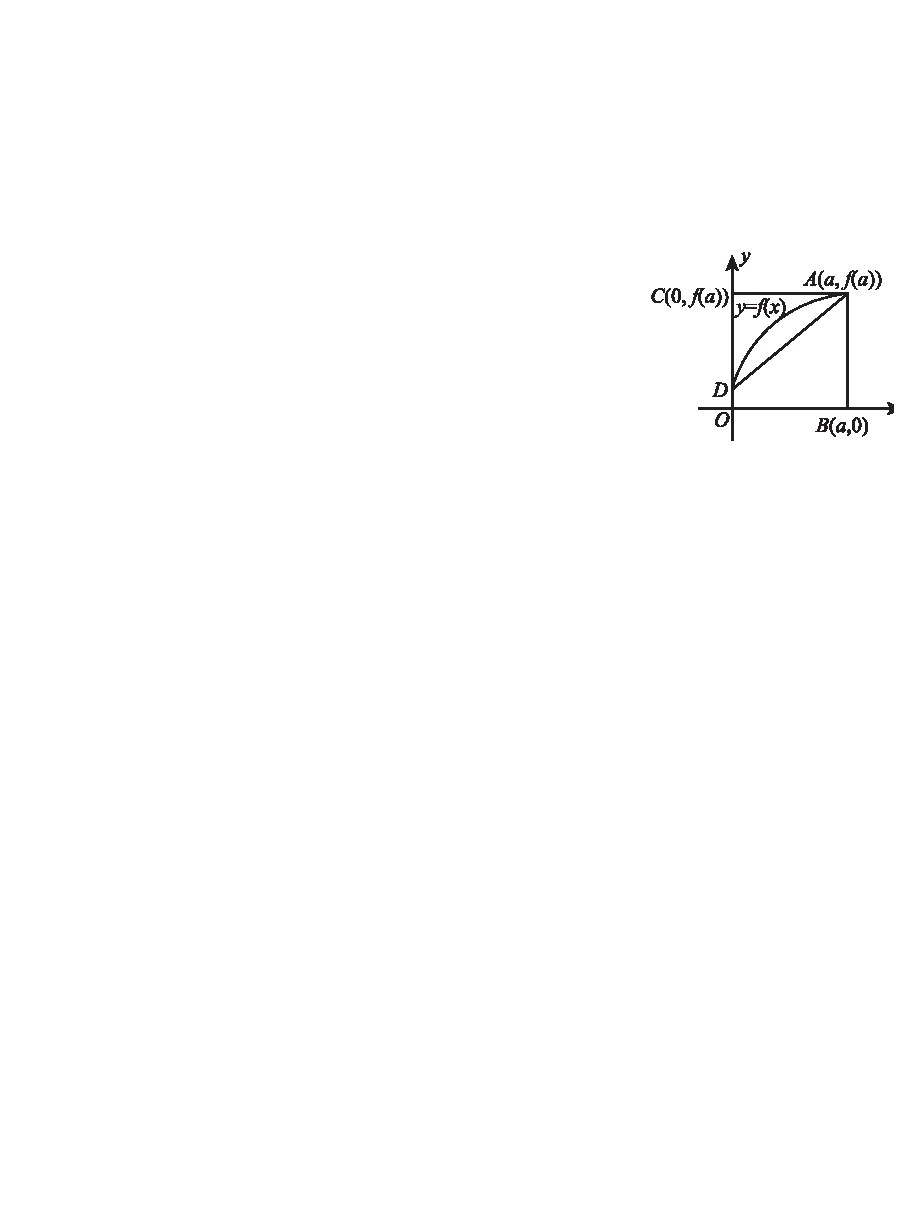
\includegraphics[width=.48\linewidth]{../assets/figures/page-113-04.pdf}\end{center}

（A）曲边梯形 \(\displaystyle ABOD\) 的面积。（B）梯形 \(\displaystyle ABOD\) 的面积。（C）曲边三角形 \(\displaystyle ACD\) 的面积。（D）三角形 \(\displaystyle ACD\) 的面积。


（3）已知 \(\displaystyle f(x,\allowbreak y)=e^{\sqrt{x^2+y^4}}\)，则（　）。（A）\(\displaystyle f_x^{\prime}(0,\allowbreak 0)\)、\(\displaystyle f_y^{\prime}(0,\allowbreak 0)\) 都存在。（B）\(\displaystyle f_x^{\prime}(0,\allowbreak 0)\) 不存在，\(\displaystyle f_y^{\prime}(0,\allowbreak 0)\) 存在。（C）\(\displaystyle f_x^{\prime}(0,\allowbreak 0)\) 存在，\(\displaystyle f_y^{\prime}(0,\allowbreak 0)\) 不存在。（D）\(\displaystyle f_x^{\prime}(0,\allowbreak 0)\)、\(\displaystyle f_y^{\prime}(0,\allowbreak 0)\) 都不存在。


（4）设函数 \(\displaystyle f\) 连续，若 \(\displaystyle F(u,\allowbreak v)=\displaystyle \iint_{D_{uv}}\dfrac{\displaystyle f(x^2+y^2)}{\displaystyle \sqrt{x^2+y^2}}\,\mathrm dx\,\mathrm dy\)，其中区域 \(\displaystyle D_{uv}\) 为图中阴影部分，则 \(\displaystyle \dfrac{\displaystyle \partial F}{\displaystyle \partial u}=\)（　）。


\begin{center}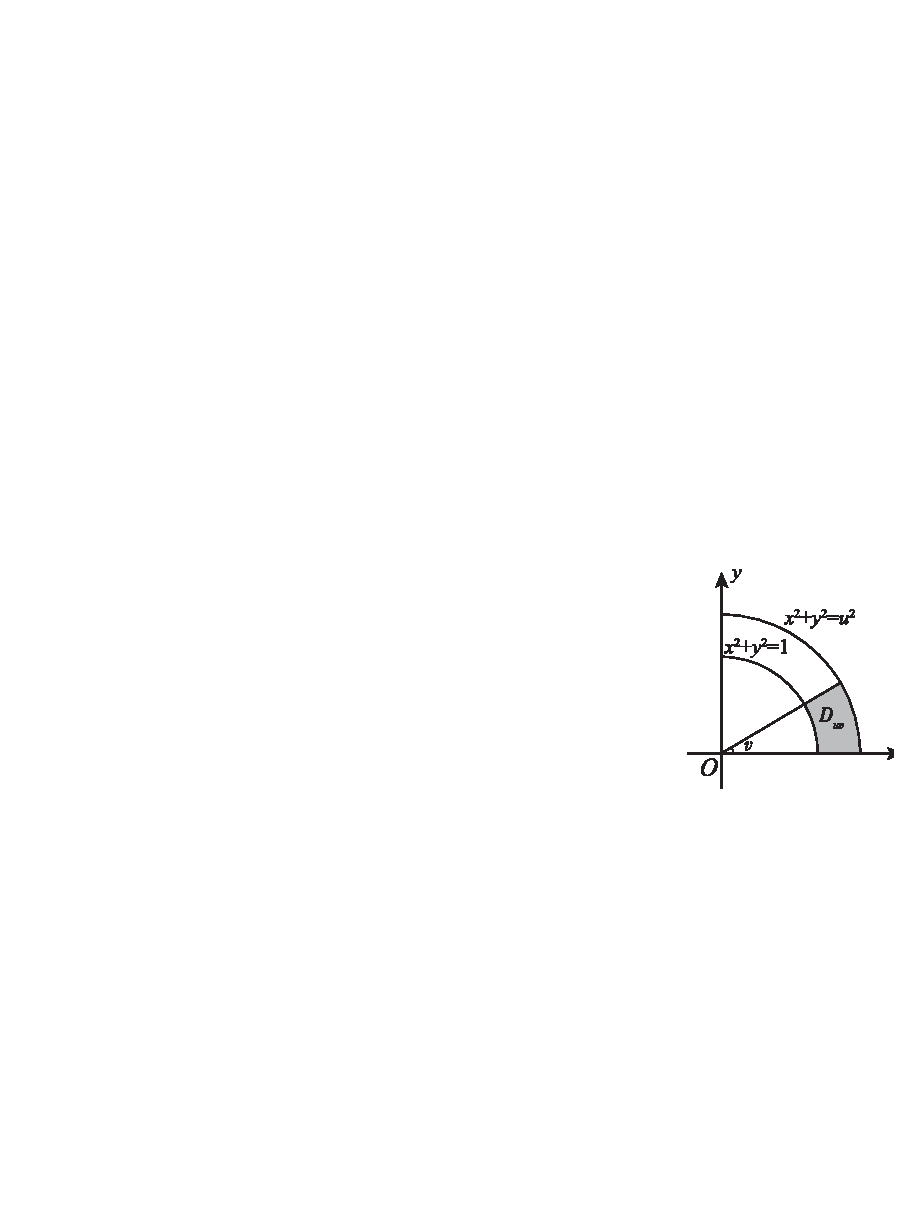
\includegraphics[width=.48\linewidth]{../assets/figures/page-113-08.pdf}\end{center}

（A）\(\displaystyle vf(u^2)\)。（B）\(\displaystyle \dfrac{\displaystyle v}{\displaystyle u} f(u^2)\)。（C）\(\displaystyle vf(u)\)。（D）\(\displaystyle \dfrac{\displaystyle v}{\displaystyle u} f(u)\)。


（5）设 \(\displaystyle A\) 为 \(\displaystyle n\) 阶非零矩阵，\(\displaystyle E\) 为 \(\displaystyle n\) 阶单位矩阵，若 \(\displaystyle A^3=O\)，则（　）。（A）\(\displaystyle E-A\) 不可逆，\(\displaystyle E+A\) 不可逆。（B）\(\displaystyle E-A\) 不可逆，\(\displaystyle E+A\) 可逆。（C）\(\displaystyle E-A\) 可逆，\(\displaystyle E+A\) 可逆。（D）\(\displaystyle E-A\) 可逆，\(\displaystyle E+A\) 不可逆。


（6）设 \(\displaystyle A=\begin{pmatrix}1&2\\2&1\end{pmatrix}\)，则在实数域上与 \(\displaystyle A\) 合同的矩阵为（　）。（A）\(\displaystyle \begin{pmatrix}-2&1\\1&-2\end{pmatrix}\)。（B）\(\displaystyle \begin{pmatrix}2&-1\\-1&2\end{pmatrix}\)。（C）\(\displaystyle \begin{pmatrix}2&1\\1&2\end{pmatrix}\)。（D）\(\displaystyle \begin{pmatrix}1&-2\\-2&1\end{pmatrix}\)。


（7）设随机变量 \(\displaystyle X,\allowbreak Y\) 独立同分布，且 \(\displaystyle X\) 的分布函数为 \(\displaystyle F(x)\)，则 \(\displaystyle Z=\displaystyle \max\{X,\allowbreak Y\}\) 的分布函数为（　）。（A）\(\displaystyle F^2(x)\)。（B）\(\displaystyle F(x)F(y)\)。（C）\(\displaystyle 1-[1-F(x)]^2\)。（D）\(\displaystyle [1-F(x)][1-F(y)]\)。


（8）设随机变量 \(\displaystyle X\sim N(0,\allowbreak 1)\)，\(\displaystyle Y\sim N(1,\allowbreak 4)\)，且相关系数 \(\displaystyle \rho_{XY}=1\)，则（　）。（A）\(\displaystyle P\{Y=-2X-1\}=1\)。（B）\(\displaystyle P\{Y=2X-1\}=1\)。（C）\(\displaystyle P\{Y=-2X+1\}=1\)。（D）\(\displaystyle P\{Y=2X+1\}=1\)。


\subsection*{二、填空题（本题共6小题，每小题4分，满分24分）}

（9）设函数 \(\displaystyle f(x)=\begin{cases}x^2+1,\allowbreak &|x|\le c,\allowbreak \\\dfrac{\displaystyle 2}{\displaystyle |x|},\allowbreak &|x|>c\end{cases}\) 在 \(\displaystyle ( -\infty,\allowbreak +\infty)\) 内连续，则 \(\displaystyle c=\)\_\_\_\_\_\_。


（10）设 \(\displaystyle f\!\left(x+\dfrac{\displaystyle 1}{\displaystyle x}\right)=\dfrac{\displaystyle x+x^3}{\displaystyle 1+x^4}\)，则 \(\displaystyle \int_2^{2\sqrt2}f(x)\,\mathrm dx=\)\_\_\_\_\_\_。


（11）设 \(\displaystyle D=\{(x,\allowbreak y)\mid x^2+y^2\le1\}\)，则 \(\displaystyle \iint_D(x^2-y)\,\mathrm dx\,\mathrm dy=\)\_\_\_\_\_\_。


（12）微分方程 \(\displaystyle xy^{\prime}+y=0\) 满足条件 \(\displaystyle y(1)=1\) 的解是 \(\displaystyle y=\)\_\_\_\_\_\_。


（13）设3阶矩阵 \(\displaystyle A\) 的特征值为 \(\displaystyle 1,\allowbreak 2,\allowbreak 2\)，\(\displaystyle E\) 为3阶单位矩阵，则 \(\displaystyle |4A^{-1}-E|=\)\_\_\_\_\_\_。


（14）设随机变量 \(\displaystyle X\) 服从参数为1的泊松分布，则 \(\displaystyle P\{X=E(X^2)\}=\)\_\_\_\_\_\_。


\subsection*{三、解答题（本题共9小题，满分94分，解答应写出文字说明、证明过程或演算步骤）}

（15）（本题满分9分）计算 \(\displaystyle \lim_{x\to0}\dfrac{\displaystyle 1}{\displaystyle x^2}\ln\dfrac{\displaystyle \sin x}{\displaystyle x}\)。


（16）（本题满分10分）设 \(\displaystyle z=z(x,\allowbreak y)\) 是由方程 \(\displaystyle x^2+y^2-z=\varphi(x+y+z)\) 所确定的函数，其中 \(\displaystyle \varphi\) 具有二阶导数，且 \(\displaystyle \varphi^{\prime}\ne-1\)。（I）求 \(\displaystyle \mathrm dz\)；（II）记 \(\displaystyle u(x,\allowbreak y)=\dfrac{\displaystyle 1}{\displaystyle x-y}\left(\dfrac{\displaystyle \partial z}{\displaystyle \partial x}-\dfrac{\displaystyle \partial z}{\displaystyle \partial y}\right)\)，求 \(\displaystyle \dfrac{\displaystyle \partial u}{\displaystyle \partial x}\)。


（17）（本题满分11分）计算 \(\displaystyle \iint_D\displaystyle \max\{xy,\allowbreak 1\}\,\mathrm dx\,\mathrm dy\)，其中 \(\displaystyle D=\{(x,\allowbreak y)\mid0\le x\le2,\allowbreak \;0\le y\le2\}\)。


（18）（本题满分10分）设 \(\displaystyle f(x)\) 是周期为2的连续函数。（I）证明对任意实数 \(\displaystyle t\)，有 \(\displaystyle \int_t^{t+2}f(x)\,\mathrm dx=\displaystyle \int_0^2f(x)\,\mathrm dx\)；（II）证明 \(\displaystyle G(x)=\displaystyle \int_0^x\left[2f(t)-\displaystyle \int_t^{t+2}f(s)\,\mathrm ds\right]\mathrm dt\) 是周期为2的周期函数。


（19）（本题满分10分）设银行存款的年利率为 \(\displaystyle r=0.05\)，并依年复利计算。某基金会希望通过存款 \(\displaystyle A\) 万元实现第一年提取19万元，第二年提取28万元，\(\displaystyle \cdots\)，第 \(\displaystyle n\) 年提取 \(\displaystyle (10+9n)\) 万元，并能按此规律一直提取下去，问 \(\displaystyle A\) 至少应为多少万元？


（20）（本题满分12分）设 \(\displaystyle n\) 元线性方程组 \(\displaystyle Ax=b\)，其中


\[\fitmath{\displaystyle A=\begin{pmatrix}2a&1&&&&\\a^2&2a&1&&&\\&a^2&2a&1&&\\&&\ddots&\ddots&\ddots&\\&&&a^2&2a&1\\&&&&a^2&2a\end{pmatrix}_{n\times n},\qquad x=\begin{pmatrix}x_1\\x_2\\\vdots\\x_n\end{pmatrix},\qquad b=\begin{pmatrix}1\\0\\\vdots\\0\end{pmatrix}.}\]


（I）证明行列式 \(\displaystyle |A|=(n+1)a^n\)；（II）当 \(\displaystyle a\) 为何值时，该方程组有唯一解，并求 \(\displaystyle x_1\)；（III）当 \(\displaystyle a\) 为何值时，该方程组有无穷多解，并求通解。


（21）（本题满分10分）设 \(\displaystyle A\) 为3阶矩阵，\(\displaystyle \alpha_1,\allowbreak \alpha_2\) 为 \(\displaystyle A\) 的分别属于特征值 \(\displaystyle -1,\allowbreak 1\) 的特征向量，向量 \(\displaystyle \alpha_3\) 满足 \(\displaystyle A\alpha_3=\alpha_2+\alpha_3\)。（I）证明 \(\displaystyle \alpha_1,\allowbreak \alpha_2,\allowbreak \alpha_3\) 线性无关；（II）令 \(\displaystyle P=(\alpha_1,\allowbreak \alpha_2,\allowbreak \alpha_3)\)，求 \(\displaystyle P^{-1}AP\)。


（22）（本题满分11分）设随机变量 \(\displaystyle X\) 与 \(\displaystyle Y\) 相互独立，\(\displaystyle X\) 的概率分布为 \(\displaystyle P\{X=i\}=\dfrac{\displaystyle 1}{\displaystyle 3}\;(i=-1,\allowbreak 0,\allowbreak 1)\)，\(\displaystyle Y\) 的概率密度为 \(\displaystyle f_Y(y)=\begin{cases}1,\allowbreak &0\le y<1,\allowbreak \\0,\allowbreak &\text{其他},\allowbreak \end{cases}\) 记 \(\displaystyle Z=X+Y\)。（I）求 \(\displaystyle P\{Z\le\dfrac{\displaystyle 1}{\displaystyle 2}\mid X=0\}\)；（II）求 \(\displaystyle Z\) 的概率密度 \(\displaystyle f_Z(z)\)。


（23）（本题满分11分）设 \(\displaystyle X_1,\allowbreak X_2,\allowbreak \cdots,\allowbreak X_n\) 是总体 \(\displaystyle N(\mu,\allowbreak \sigma^2)\) 的简单随机样本，记 \(\displaystyle \bar X=\dfrac{\displaystyle 1}{\displaystyle n}\displaystyle \sum_{i=1}^nX_i\)，\(\displaystyle S^2=\dfrac{\displaystyle 1}{\displaystyle n-1}\displaystyle \sum_{i=1}^n(X_i-\bar X)^2\)，\(\displaystyle T=\bar X^2-\dfrac{\displaystyle 1}{\displaystyle n}S^2\)。（I）（超纲题）证明 \(\displaystyle T\) 是 \(\displaystyle \mu^2\) 的无偏估计量。（无偏估计为超纲概念，可改为“证明 \(\displaystyle E(T)=\mu^2\)”）；（II）当 \(\displaystyle \mu=0,\allowbreak \sigma=1\) 时，求 \(\displaystyle D(T)\)。

\end{document}
